
\documentclass{article}

\usepackage{amssymb}
\usepackage{amsmath}
\usepackage{txfonts}
\usepackage{mathdots}
\usepackage{titlesec}
\usepackage{array}
\usepackage{lastpage}
\usepackage{etoolbox}
\usepackage{tabularray}
\usepackage{color, colortbl}
\usepackage{adjustbox}
\usepackage{geometry}
\usepackage[classicReIm]{kpfonts}
\usepackage{hyperref}
\usepackage{fancyhdr}

\usepackage{float}
\usepackage{setspace}
\restylefloat{table}
\usepackage{graphicx}
\usepackage[table]{xcolor}
\graphicspath{ {./slike/} }


\linespread{1.3} %razmak između redaka

\geometry{a4paper, left=1in, top=1in,}  %oblik stranice

\hypersetup{ colorlinks, citecolor=black, filecolor=black, linkcolor=black,	urlcolor=black }   %izgled poveznice

%Promjena teksta za dugačke tablice
\DefTblrTemplate{contfoot-text}{normal}{Nastavljeno na idućoj stranici}
\SetTblrTemplate{contfoot-text}{normal}
\DefTblrTemplate{conthead-text}{normal}{(Nastavljeno)}
\SetTblrTemplate{conthead-text}{normal}
\DefTblrTemplate{middlehead,lasthead}{normal}{Nastavljeno od prethodne stranice}
\SetTblrTemplate{middlehead,lasthead}{normal}

%podesavanje zaglavlja i podnožja

\pagestyle{fancy}
\lhead{Programsko inženjerstvo}
\rhead{Šahisti}
\lfoot{AlmostByte}
\cfoot{\thepage}
\rfoot{\today}
\renewcommand{\headrulewidth}{0.2pt}
\renewcommand{\footrulewidth}{0.2pt}
\begin{document}

\newenvironment{packed_enum}{
	\begin{enumerate}
		\setlength{\itemsep}{0pt}
		\setlength{\parskip}{0pt}
		\setlength{\parsep}{0pt}
	}{\end{enumerate}}

\newenvironment{packed_item}{
	\begin{itemize}
		\setlength{\itemsep}{0pt}
		\setlength{\parskip}{0pt}
		\setlength{\parsep}{0pt}
	}{\end{itemize}}
	
		\begin{titlepage}
		\begin{center}
			\vspace*{\stretch{1.0}} %u kombinaciji s ostalim \vspace naredbama definira razmak između redaka teksta
			\LARGE Programsko inženjerstvo\\
			\large Ak. god. 2022./2023.\\
			
			\vspace*{\stretch{3.0}}
			
			\huge Šahisti\\
			\Large Dokumentacija, Rev. \textit{1}\\
			
			\vspace*{\stretch{12.0}}
			\normalsize
			Grupa: \textit{AlmostByte}\\
			Voditelj: \textit{Ivan Bilobrk}\\
			
			
			\vspace*{\stretch{1.0}}
			Datum predaje: \textit{18. 11. 2022.}\\
			
			\vspace*{\stretch{4.0}}
			
			Nastavnik: \textit{$<$Ime i prezime nastavnika zaduženog za vašu grupu$>$}\\
			
		\end{center}
		
		
	\end{titlepage}

	\tableofcontents
	\eject
		
	\section{Dnevnik promjena dokumentacije}	
		\begin{longtblr}[
		label=none
		]{
			width = \textwidth, 
			colspec={|X[2]|X[13]|X[3]|X[3]|}, 
			rowhead = 1
		}
		\hline
		\textbf{Rev.}	& \textbf{Opis promjene/dodatka} & \textbf{Autori} & \textbf{Datum}\\[3pt] \hline
		0.1 & Preuzet predložak i izrađena gruba kopija predloška dokumentacije.	& Anteo Vukasović & 15.10.2022. 		\\[3pt] \hline 
		0.2	& Napisan i dodan opis use caseova.& Anteo Vukasović & 29.10.2022.	\\[3pt] \hline 
		0.3 & Napisani i dodani funkcionalni zahtjevi.  & Anteo Vukasović & 03.11.2022. \\[3pt] \hline 
		0.4 & Dodani use case dijagrami. & Mijo Rajič & 05.11.2022. \\[3pt] \hline 
		0.5 & Napisan i dodan opis projektnog zadatka. & Anteo Vukasović & 06.11.2022. \\[3pt] \hline 
		0.6 & Dodani sekvencijski dijagrami te njihovi opisi. & Altea Božić, Tina Jureško i Lara \newline Mahalec & 09.11.2022. \\[3pt] \hline 
		0.7 & Napisan i dodan opis baze podataka. &  Lara \newline Mahalec & 11.11.2022. \\[3pt] \hline
		0.8 & Napisan i dodan opis arhitekture sustava. & Anteo Vukasović & 17.11.2022. \\[3pt] \hline
		0.10 & Kompletirana tablica promjena dokumentacije za prvi ciklus. & Anteo Vukasović & 18.11.2022. \\[3pt] \hline  
		\textbf{1.0} & Verzija samo s bitnim dijelovima za 1. ciklus & \textit{verificirao \newline cijeli tim} & 18.11.2022. \\[3pt] \hline 
	\end{longtblr}

	\eject
	
	\section{Opis projektnog zadatka}
		Cilj ovog projektnog zadatka je izrada funkcionalne web aplikacije koju će koristiti članovi šahovskog kluba. Ova web aplikacija olakšala bi trenerima u šahovskom klubu organizaciju i vodenje treninga i natjecanja svojih učenika, a učenicima bi pružila platformu na kojoj bi mogli okušati svoja znanja i vještine putem dnevnih taktika. Na taj način svi korisnici mogu doraditi i unaprijediti svoja znanja i vještine u divnoj šahovskoj igri. \\ 
		Aplikacija je dizajnirana primarno za članove šahovskog kluba, samo oni će imati pristup punoj funkcionalnosti aplikacije. No to ne sprječava sve one zainteresirane da dobiju uvid u svijet šaha putem ove aplikacije. \\
		Prilikom pokretanja same aplikacije, korisnika se vodi na stranicu s 3 opcije:
		\begin{itemize}
			\item Registracija
			\item Prijava u sustav
			\item  Nastavi kao gost
		\end{itemize}
		Ukoliko korisnik želi nastaviti bez ikakve prijave ili registracije te odabere posljednju opciju, vodi ga se na početnu stranicu koja ne nudi sve opcije kao što bi u normalnom načinu rada, no ipak nudi dosta zabavnog sadržaja. Korisnik u ovom načinu rada može:
		\begin{itemize}
			\item Riješiti dnevnu taktiku 
			\item Pročitati novosti i zanimljivosti 
			\item Pregledati rang listu članova 
		\end{itemize}
		Novosti i zanimljivosti je rubrika koju treneri ureduju po svojoj volji. Koncipirana je kao svojevrsna lista članaka čiji sadržaj bi bile vijesti o radu i rezultatima kluba, vijesti iz svijeta šaha i šahovskih natjecanja diljem svijeta, crtice iz povijesti, analize legendarnih šahovskih partija i slično. 
		
		Dnevna taktika je kratka šahovska zagonetka, najčešće od 1 do 5 poteza, u kojoj je cilj naći optimalnu kombinaciju poteza u danom scenariju šahovske igre. Primjer jedne takve zagonetke možemo vidjeti na raznim šahovskim platformama kao što su lichess(link), chess.com(link) i slični. U našoj aplikaciji, dnevna taktika bilježi vrijeme rješavanja, te točnost ponudenog rješenja. Rješavanjem dnevne taktike, neregistriranog korisnika se obavijesti o ispravnosti njegova rješenja, no njegovo rješenje se nigdje ne pohranjuje, niti taj korisnik sam može biti uvršten u rang listu. Za te funkcionalnosti korisnik mora biti član, a član može postati registracijom.\\
		
		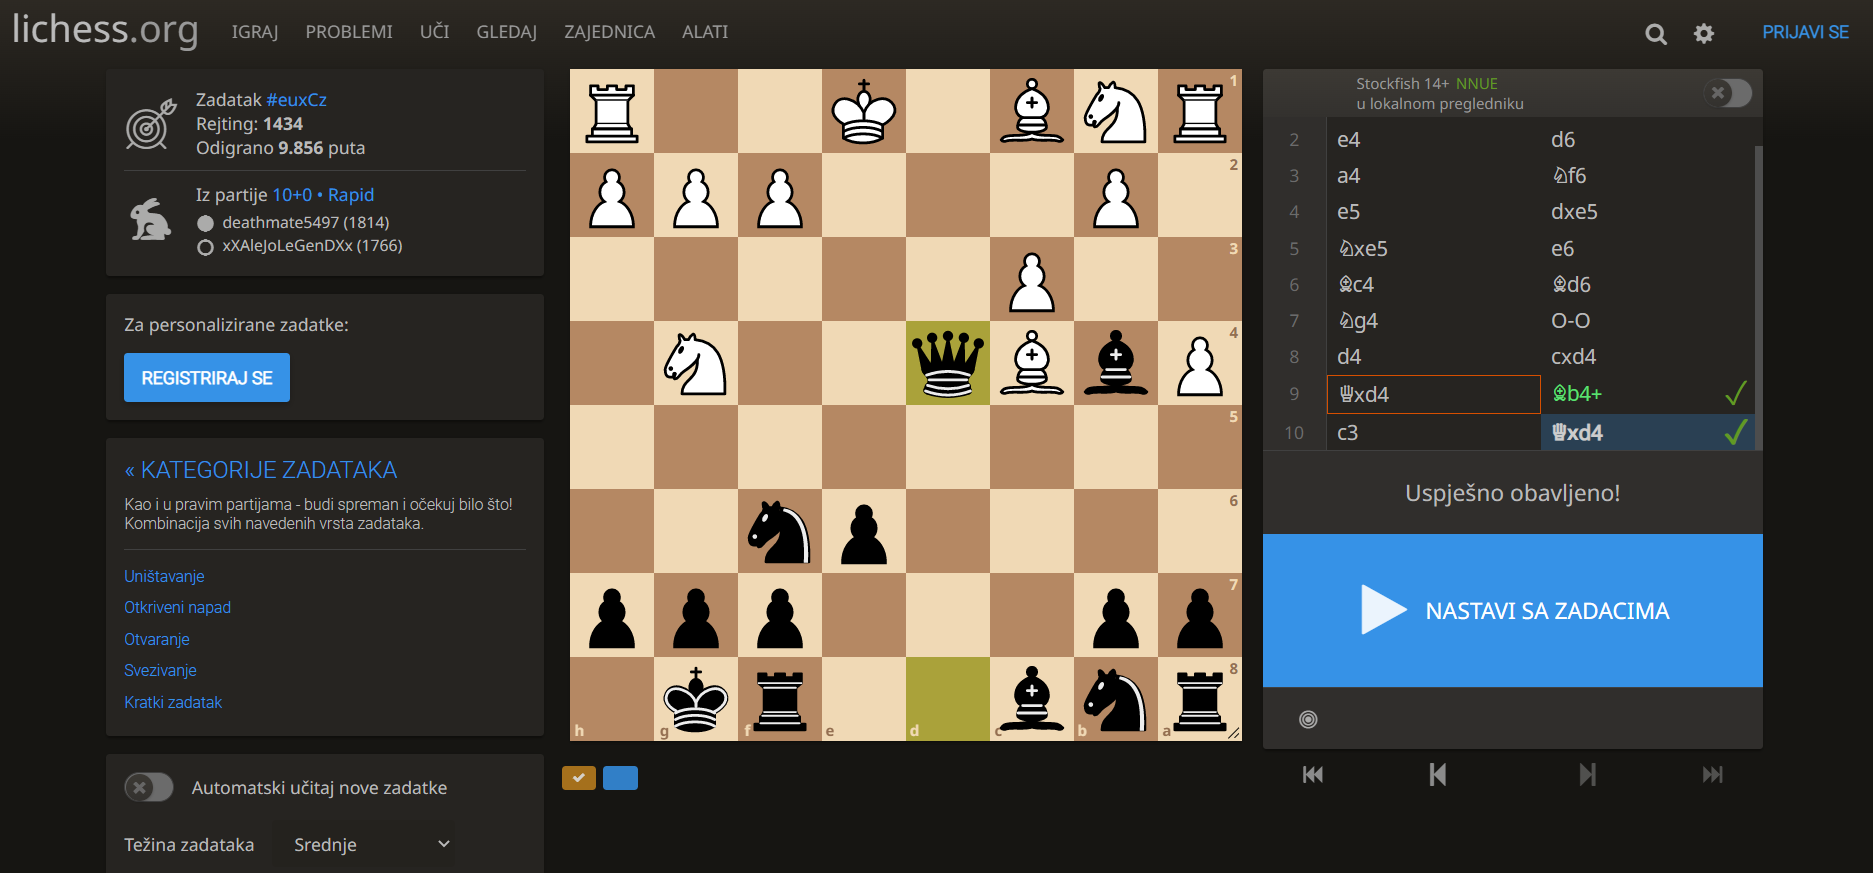
\includegraphics[width=\columnwidth]{lichess_primjer}
		\begin{center}
			\textit{Slika 2.1: Primjer šahovske zagonetke}
		\end{center}
		
		Registracija nudi korisnicima koji žele postati članovi šahovskog kluba mogućnost da tu želju ostvare. Odabirom te opcije korisnika se vodi na formular u kojem korisnik unosi svoje vlastite podatke. Ukoliko su svi podatci ispravno uneseni, korisnik se pohranjuje u bazu podataka te postaje punopravni član šahovskog kluba. Čestitke!
		
		Prijava u sustav je slična registraciji, jedina razlika je ta što njoj pristupaju postojeći članovi kluba, stoga moraju unijeti ispravne podatke koji već postoje u bazi podataka šahovskog kluba kako bi im se omogućio pristup aplikaciji. 
		
		Ukoliko je korisnik prijavljen u sustav te se radi o članu šahovskog kluba koji nije trener, korisnik u aplikaciji može: 
		\begin{itemize}
			\item Pregledati osobne podatke 
			\item Riješiti dnevnu taktiku 
			\item Pročitati novosti i zanimljivosti 
			\item Pregledati rang listu članova 
			\item Prijaviti se na treninge 
			\item Prijaviti se na turnire
			\item Biti dio rang liste svih članova 
			\item Prijaviti rješenja dnevne taktike 
			\item Platiti članarinu i pregledati svoja prijašnja plaćanja 
		\end{itemize}
		
		Treća i četvrta točka prethodne liste se ne razlikuju prema funkcionalnosti od funkcionalnosti koju za iste komponente imaju neregistrirani članovi. 
		
		Rješavanje dnevne taktike je isto kao i kod neregistriranih korisnika, no ono što se odvija nakon samog rješavanja jest drugačije. Kod registriranih članova, rješenja se pohranjuju u bazu podataka. Na temelju toga kreira se rang lista svih članova kluba. Rang lista uzima u obzir sve riješene taktike te 3 parametra tih rješenja; točnost, brzinu i težinu same taktike. 
		
		Osim rješavanja dnevne taktike članovi imaju opciju prijavljivanja rješenja. Ukoliko smatraju kako rješenje nije ispravno, korisnici odabiru opciju za prijavu dnevne taktike te obavljaju proces podnošenja prijave koji se sastoji od 3 koraka: 
		\begin{packed_enum}
			\item Unos novih poteza za koje član smatra da su ispravni 
			\item Tekstualni opis tih rješenja, iznošenje svojih misli iza priloženih novih rješenja 
			\item Odabir trenera kojem se šalje zahtjev 
		\end{packed_enum}
		Ukoliko trener prihvati novo rješenje, ono se uzima kao ispravno te se rang liste ažuriraju prema ovim rješenjima.  
		
		Član se unutar naše aplikacije može prijavljivati na treninge i turnire objavljene na aplikaciju od strane trenera. Odabirom opcije za prijavu na turnir/trening, član odlazi na stranicu gdje vidi popis svih dostupnih treninga i turnira. Ukoliko nema nikakvih konflikata ili prekršenih ograničenja o maksimalnom broju dopuštenih članova u treningu/turniru, člana se prijavljuje na dani trening/turnir. 
		
		Odabirom opcije za pregled osobnih podataka, član na jednom mjestu vidi svoje osnovne osobne podatke koje je unio u trenutku registracije te svu svoju aktivnost na aplikaciji. 
		
		Svaki član mora platiti članarinu kako bi mogao i dalje biti punopravni član, a naša aplikacija nudi opciju plaćanja. Odabirom opcije za plaćanje članarine, člana se vodi na popis svih svojih računa. Ukoliko na tom popisu ima neplaćenih, člana se o tome obavijesti te odabirom pojedinog neplaćenog računa korisnik može platiti taj račun unošenjem osnovnih podataka potrebnih za plaćanje. Za člana je bitno da uredno plaća svoje račune jer je moguće da mu administrator(više o njemu kasnije) ograniči pristup aplikaciji sve dok ne plati sve neplaćene članarine.\\ 
		
		
		Osim članova, u šahovskom klubu postoje i treneri. Oni su zaduženi za objavljivanje sadržaja i aktivnosti na aplikaciju koje članovi kasnije mogu koristiti. Treneri na aplikaciji mogu:
		
		\begin{itemize}
			\item Pregledati osobne podatke 
			\item Objavljivati i ažurirati dnevne taktike 
			\item Objavljivati novosti i zanimljivosti 
			\item Objavljivati treninge 
			\item Organizirati i objaviti turnire 
			\item Revidirati zaprimljene prijave o neispravnim rješenjima dnevnih taktika 
		\end{itemize} 
		
		Prva točka je identična kao kod članova, iste funkcionalnosti imaju i jedni i drugi. 
		
		Treneri mogu objavljivati novosti i zanimljivosti na aplikaciju te postavljati nove dnevne taktike. Kod svake od navedenih rubrika u aplikaciji, za trenere će biti ponudena opcija dodavanja novog sadržaja. Primjerice, kod unosa novosti, treneru će se otvoriti prostor za unošenje teksta u kojem trener upisuje što želi. Nakon što je gotov, trener potvrdi svoju namjeru objavljivanja odabirom prikladnog gumba te se taj tekst dodaje u aplikaciju. 
		
		Treninge i turnire trener dodaje odabirom opcije za dodavanje novog treninga/turnira. Odabire termin početka i vrijeme trajanja te potencijalno ograničenje maksimalnog broja sudionika. Ukoliko su svi kriteriji zadovoljeni, aktivnost se dodaje u bazu podataka i prikazuje se unutar aplikacije. Ukoliko termin nije ispravan te dolazi do kolizije s nekom drugom aktivnosti, trenera se vraća na ponovni odabir ispravnog termina. 
		
		U prijašnjem dijelu teksta smo vidjeli kako članovi mogu prijavljivati dnevne taktike za koje misle da imaju bolja rješenja od onih koja su ponudena. Odabirom na opciju pristigle prijave, trener može pregledati imaju li kakvih prijava od članova. Ukoliko imaju, mogu pogledati cijeli tekst prijave i proučiti ponovno dnevnu taktiku. Smatraju li kako je prijava neutemeljena treneri je samo odbacuju. Na ako je prijava valjana, trener može promijeniti rješenje dnevne taktike te ju na taj način ažurirati. Tim činom se ujedno i ažuriraju rang liste.\\ 
		
		
		Osim do sada navedenih korisnika aplikacije, postoji i još jedna vrsta korisnika a to je administrator. Njegove ovlasti su slične kao kod trenera, no još dodatno proširene. On može vidjeti sav sadržaj aplikacije, ali može ga i ukloniti i mijenjati po volji, bez obzira je li on autor tog sadržaja. Uz to, administrator ima opciju zabrane pristupa korisnicima. Ova akcija se može dogoditi iz proizvoljnih razloga no istaknimo jedan poseban scenarij; član uredno ne plaća svoju članarinu. Administrator može vidjeti pregled svih plaćanja svakog člana te ako utvrdi da pojedini član ima previše neplaćenih računa može mu ograničiti pristup aplikaciji. Taj član će od funkcionalnosti jedino moći vidjeti svoja plaćanja i platiti svoje neplaćene račune, i tako sve dok ne plati račune. U tom slučaju, administrator može maknuti restrikcije tom članu.
		\eject 
		
	\section{Specifikacija programske potpore}
		\subsection{Funkcionalni zahtjevi}
		\textit{Dionici ovog sustava su predsjednik šahovskog kluba, administrator sustava, razvojni tim te članovi kluba}\\
		
		\noindent \textit{Aktori ovog sustava su neregistrirani korisnici, registrirani članovi, registrirani treneri te administratori kao inicijatori, te baza podataka kao sudionik. }\\
		
		\noindent \textbf{Dionici:}
		
		\begin{packed_enum}
			
			\item Predsjednik kluba (naručitelj) 
			\item Članovi kluba 
			\begin{packed_enum}
				\item Treneri
				\item Polaznici
			\end{packed_enum}
			\item Administrator 
			\item Razvojni tim 
			
		\end{packed_enum}
	
		\noindent \textbf{Aktori:}
		\begin{packed_enum}
			\item Neregestrirani korisnik(inicijator) može:
			\begin{packed_enum}
				\item Obaviti registraciju i postati članom kluba 
				\item Pregledati novosti postavljene od strane trenera/administratora na aplikaciju 
				\item Rješavati dnevnu taktiku 
				\item Vidjeti rang listu uspješnosti rješavanja dnevnih taktika svih članova
			\end{packed_enum}
			\item Registrirani član(inicijator) može:
			\begin{packed_enum}
				\item Pregledati svoje osobne podatke 
				\item Obaviti plaćanje i pregled računa(članarine) 
				\item Prijaviti se na treninge postavljene na stranicu od strane trenera 
				\item Prijaviti se na turnire postavljene na stranicu od strane trenera
				\item Rješavati dnevne taktike uz pohranjivanje rješenja u bazu podataka te ažuriranje rang liste svih članova na temelju točnosti i brzine rješavanja taktike 
				\item Prijaviti greške u dnevnoj taktici na način da unese i opiše nove poteze za koje smatra da su pravo rješenje te pošalje svoja zapažanja proizvoljnom treneru na reviziju 
			\end{packed_enum}
			\item Trener(inicijator) može:
			\begin{packed_enum}
				\item Pregledati svoje osobne podatke 
				\item Postavljati nove dnevne taktike na aplikaciju 
				\item Postavljati novosti na aplikaciju 
				\item Postavljati raspored svojih treninga na aplikaciju te omogućiti članovima prijavu na iste 
				\item Organizirat turnire za članove te omogućiti članovima prijavu na iste 
				\item Revidirati zaprimljene prijave pogreški u dnevnim taktikama te ukoliko je potrebno ažurirati ih 
			\end{packed_enum}
			\item Administrator(incijator) može:
			\begin{packed_enum}
				\item Imati uvid u sve podatke na aplikaciji te opciju uredivanja i dodavanja novih sadržaja
				\item Zabraniti pristup aplikaciji odredenim članovima/trenerima 
				\item Pregledati plaćanja svih članova te ukoliko ima neplaćenih računa odredenim članovima zabraniti pristup dok ne obavi plaćanja
			\end{packed_enum}
			\item Baza podataka(sudionik):
			\begin{packed_enum}
				\item Pohranjuje sve osobne podatke o registriranim članovima
				\item Pohranjuje sve akcije registriranih članova
				\item Pohranjuje status o potencijalnoj zabrani pristupa nekom od članova
			\end{packed_enum}
		\end{packed_enum}
		\eject
		
		\subsubsection{Obrasci uporabe}
		\noindent \textbf{Opis obrazaca uporabe:}\\
		
		\noindent {\textbf{UC1 - Registracija}}
		\begin{packed_item}
			
			\item \textbf{Glavni sudionik: }Neregistrirani korisnik
			\item  \textbf{Cilj:} Stvaranje korisničkog računa za neregistriranog korisnika
			\item  \textbf{Sudionici:} Baza podataka
			\item  \textbf{Preduvjet:} -
			\item  \textbf{Opis osnovnog tijeka:}
			
			\item[] \begin{packed_enum}
				\item Odabir gumba za registraciju
				\item Ispunjavanje ponudenog formulara
				\item Pohranjivanje podataka u bazu podataka
				\item Otvaranje početne stranice 
			\end{packed_enum}
			
			\item  \textbf{Opis mogućih odstupanja:}
			
			\item[] \begin{packed_item}
				
				\item[2.a] Odabir već zauzetog korisničkog imena i/ili e-maila, unos korisničkog podatka u nedozvoljenom formatu ili pružanje neispravnoga e-maila
				\item[] \begin{packed_enum}
					\item Sustav obavještava korisnika o greški i vraća ga na registraciju 
					\item Korisnik ispravlja grešku i uspješno obavlja registraciju ili ne uspijeva dok ne odustane
				\end{packed_enum}
			\end{packed_item}
		\end{packed_item}
	
		\noindent {\textbf{UC2 - Prijava u sustav}}
		\begin{packed_item}
			
			\item \textbf{Glavni sudionik: }Registrirani korisnik
			\item  \textbf{Cilj:} Verifikacija postojanja korisničkog računa i mogućnost pristupa većem broju sadržaja na stranici
			\item  \textbf{Sudionici:} Baza podataka
			\item  \textbf{Preduvjet:} -
			\item  \textbf{Opis osnovnog tijeka:}
			
			\item[] \begin{packed_enum}
				\item Odabir gumba za prijavu u sustav 
				\item Popunjavanje danog formulara 
				\item Provjera postojanja danih podataka u samoj bazi podataka 
				\item Otvaranje početne stranice 
			\end{packed_enum}
			
			\item  \textbf{Opis mogućih odstupanja:}
			
			\item[] \begin{packed_item}
				
				\item[2.a] Korisniku je onemogućen pristup aplikaciji
				\item[2.b] Unos neispravnog korisničkog imena ili lozinke 
				\item[] \begin{packed_enum}
					\item Sustav obavještava korisnika o greški i vraća ga na prijavu u sustav  
					\item Korisnik ispravlja grešku i uspješno obavlja registraciju ili ne uspijeva dok ne odustane
				\end{packed_enum}
			\end{packed_item}
		\end{packed_item}	
		
		\noindent {\textbf{UC3 - Pregled novosti}}
		\begin{packed_item}
			
			\item \textbf{Glavni sudionik: }Korisnik
			\item  \textbf{Cilj:} Mogućnost pregledavanja novosti postavljenih na stranicu od strane ovlaštenih korisnika(trener/admin)
			\item  \textbf{Sudionici:} Baza podataka
			\item  \textbf{Preduvjet:} -
			\item  \textbf{Opis osnovnog tijeka:}
			
			\item[] \begin{packed_enum}
				\item Korisnik otvaranjem glavne stranice vidi sve novosti postavljene na stranici  
				\item Klikom na novost dobiva potpuni pregled same novosti  
			\end{packed_enum}
		\end{packed_item}	
		
				\noindent {\textbf{UC4 - Rješavanje dnevne taktike}}
		\begin{packed_item}
			
			\item \textbf{Glavni sudionik: }Korisnik
			\item  \textbf{Cilj:}  Otvaranje postavljene dnevne taktike i prijavljivanje rješenja
			\item  \textbf{Sudionici:} Baza podataka
			\item  \textbf{Preduvjet:} -
			\item  \textbf{Opis osnovnog tijeka:}
			
			\item[] \begin{packed_enum}
				\item Otvaranje dnevne taktike i prikaz prosječne ocjene taktike 
				\item Prijava rješenja i njegova pohrana u bazu podataka te ažuriranje rang listi(pohrana i ažuriranje samo ako je korisnik registriran) 
				\item Nakon predaje rješenja korisnik dobije obavijest o točnosti rješenja te točno rješenje ukoliko ga sam nije ponudio  
			\end{packed_enum}
		\end{packed_item}	
		
		\noindent {\textbf{UC5 - Pregled rang-liste}}
		\begin{packed_item}
			
			\item \textbf{Glavni sudionik: }Korisnik
			\item  \textbf{Cilj:}  Pregled težinske liste temeljene na točnosti i brzini rješavanja dnevnih taktika. Rang-lista sastavljena je od svih članova. 
			\item  \textbf{Sudionici:} Baza podataka
			\item  \textbf{Preduvjet:} -
			\item  \textbf{Opis osnovnog tijeka:}
			
			\item[] \begin{packed_enum}
				\item Korisnik pritiskom na gumb odlazi na stranicu rang-liste 
				\item Otvara mu se popis svih članova sortiranih na temelju točnosti i brzini rješavanja dnevnih taktika 
			\end{packed_enum}
		\end{packed_item}
		
		\noindent {\textbf{UC6 - Pregled osobnih podatka}}
		\begin{packed_item}
			
			\item \textbf{Glavni sudionik: }Registrirani korisnik
			\item  \textbf{Cilj:} Pregled osobnih podatka
			\item  \textbf{Sudionici:} Baza podataka
			\item  \textbf{Preduvjet:} Korisnik je prijavljen u sustav
			\item  \textbf{Opis osnovnog tijeka:}
			
			\item[] \begin{packed_enum}
				\item Korisnik odabire gumb za prikaz osobnih podataka i aktivnosti na stranici 
				\item Podatci se prikazuju u aplikaciji 
			\end{packed_enum}
		\end{packed_item}		
		
		\noindent {\textbf{UC7 - Plaćanje članarine}}
		\begin{packed_item}
			
			\item \textbf{Glavni sudionik: }Član
			\item  \textbf{Cilj:} Član plaća svoj mjesečni iznos članarine 
			\item  \textbf{Sudionici:} Baza podataka
			\item  \textbf{Preduvjet:} Korisnik je prijavljen u sustav\\
			\item  \textbf{Opis osnovnog tijeka:}
			
			\item[] \begin{packed_enum}
				\item Korisnik odabire gumb za plaćanje članarine  
				\item Na otvorenoj stranici se prikazuju neplaćeni računi(ukoliko ih ima) 
				\item Korisnik odabere račun te potvrdi plaćanje 
			\end{packed_enum}
		\end{packed_item}		
		
		\noindent {\textbf{UC8 - Prijava na trening}}
		\begin{packed_item}
			
			\item \textbf{Glavni sudionik: }Član
			\item  \textbf{Cilj:} Prijavljivanje korisnika na odabrani trening 
			\item  \textbf{Sudionici:} Baza podataka
			\item  \textbf{Preduvjet:} Korisnik je prijavljen u sustav
			\item  \textbf{Opis osnovnog tijeka:}
			
			\item[] \begin{packed_enum}
				\item Korisnik odabire gumb za prijave na treninge  
				\item Aplikacija prikazuje popis dostupnih treninga iz baze podataka  
				\item Korisnik odabire trening i njegov odabir se pohranjuje u bazu podataka 
			\end{packed_enum}
		\end{packed_item}
	
		\noindent {\textbf{UC9 - Prijava na turnir}}
		\begin{packed_item}
			
			\item \textbf{Glavni sudionik: }Član
			\item  \textbf{Cilj:} Prijavljivanje korisnika na odabrani turnir 
			\item  \textbf{Sudionici:} Baza podataka
			\item  \textbf{Preduvjet:} Korisnik je prijavljen u sustav
			\item  \textbf{Opis osnovnog tijeka:}
			
			\item[] \begin{packed_enum}
				\item Korisnik odabire gumb za prijave na turnire  
				\item Aplikacija prikazuje popis dostupnih turnira iz baze podataka  
				\item Korisnik odabire turnir i njegov odabir se pohranjuje u bazu podataka 
			\end{packed_enum}
		\end{packed_item}

		\noindent {\textbf{UC10 - Dodjeljivanje ocjene dnevnoj taktici}}
		\begin{packed_item}
			
			\item \textbf{Glavni sudionik: }Član
			\item  \textbf{Cilj:} Dodjeljivanje ocjene dnevnoj taktici od strane člana 
			\item  \textbf{Sudionici:} Baza podataka
			\item  \textbf{Preduvjet:} Korisnik je prijavljen u sustav te je riješio dnevnu taktiku 
			\item  \textbf{Opis osnovnog tijeka:}
			
			\item[] \begin{packed_enum}
				\item Nakon rješavanja dnevne taktike korisniku se otvara opcija ocjenjivanja taktike   
				\item Korisnik unosi ocjenu koja se zatim pohranjuje u bazu podataka  
			\end{packed_enum}
		\end{packed_item}
	
		\noindent {\textbf{UC11 - Prijava pogreške}}
		\begin{packed_item}
			
			\item \textbf{Glavni sudionik: }Član
			\item  \textbf{Cilj:} Član prijavljuje pogrešku u taktici ukoliko smatra da postoji optimalnije rješenje  
			\item  \textbf{Sudionici:} Baza podataka
			\item  \textbf{Preduvjet:} Korisnik je prijavljen u sustav te je riješio dnevnu taktiku 
			\item  \textbf{Opis osnovnog tijeka:}
			
			\item[] \begin{packed_enum}
				\item Korisniku se nakon rješavanja taktike nudi opcija prijavljivanja pogreške   
				\item Korisnik odabire gumb te se otvara forma za prijavljivanje pogreške 
				\item Nakon ispunjavanja forme, korisnik podnosi zahtjev za promjenom taktike koji se može odobriti ili odbiti  
			\end{packed_enum}
		\end{packed_item}
		
		\noindent {\textbf{UC12 - Unos novih poteza }}
		\begin{packed_item}
			
			\item \textbf{Glavni sudionik: }Član
			\item  \textbf{Cilj:} Korisnik predlaže nove poteze kao rješenje   
			\item  \textbf{Sudionici:} Baza podataka
			\item  \textbf{Preduvjet:} Korisnik je prijavljen u sustav te je riješio dnevnu taktiku 
			\item  \textbf{Opis osnovnog tijeka:}
			
			\item[] \begin{packed_enum}
				\item Nakon odabira prijavljivanja greške korisnik unosi svoje nove poteze kao rješenja  
			\end{packed_enum}
		\end{packed_item}
	
		\noindent {\textbf{UC13 - Opis novih poteza }}
		\begin{packed_item}
			
			\item \textbf{Glavni sudionik: }Član
			\item  \textbf{Cilj:} Korisnik daje obrazloženje predloženog rješenja taktike   
			\item  \textbf{Sudionici:} Baza podataka
			\item  \textbf{Preduvjet:} Korisnik je prijavljen u sustav te je riješio dnevnu taktiku 
			\item  \textbf{Opis osnovnog tijeka:}
			
			\item[] \begin{packed_enum}
				\item Nakon unesenih novih poteza korisnik daje pismeno objašnjenje tih poteza  
			\end{packed_enum}
		\end{packed_item}
	
		\noindent {\textbf{UC14 - Odabir trenera za revidiranje }}
		\begin{packed_item}
			
			\item \textbf{Glavni sudionik: }Član
			\item  \textbf{Cilj:} Korisnik odabire trenera koji će pregledati njegov prijedlog o promjeni taktike    
			\item  \textbf{Sudionici:} Baza podataka
			\item  \textbf{Preduvjet:} Korisnik je prijavljen u sustav te je riješio dnevnu taktiku 
			\item  \textbf{Opis osnovnog tijeka:}
			
			\item[] \begin{packed_enum}
				\item Nakon predanog opisa poteza korisniku se otvara opcija odabira medu trenerima u bazi 
				\item Korisnik odabire trenera kojem zatim dolazi taj isti zahtjev za revizijom  
			\end{packed_enum}
		\end{packed_item}
		
		\noindent {\textbf{UC15 - Postavljanje dnevne taktike  }}
		\begin{packed_item}
			
			\item \textbf{Glavni sudionik: }Trener
			\item  \textbf{Cilj:} Trener postavlja dnevnu taktiku koju ostali korisnici zatim mogu rješavati    
			\item  \textbf{Sudionici:} Baza podataka
			\item  \textbf{Preduvjet:} Korisnik je prijavljeni trener 
			\item  \textbf{Opis osnovnog tijeka:}
			
			\item[] \begin{packed_enum}
				\item Trener kreira dnevnu taktiku s njenim zadanim rješenjima  
				\item Postavljanje taktike na stranicu te njeno pohranjivanje u bazu podataka 
			\end{packed_enum}
		\end{packed_item}
		
		\noindent {\textbf{\\UC16 - Slaganje rasporeda vlastitih treninga   }}
		\begin{packed_item}
			
			\item \textbf{Glavni sudionik: }Trener
			\item  \textbf{Cilj:} Trener odabire termine treninga i postavlja ih na aplikaciju   
			\item  \textbf{Sudionici:} Baza podataka
			\item  \textbf{Preduvjet:} Korisnik je prijavljeni trener 
			\item  \textbf{Opis osnovnog tijeka:}
			
			\item[] \begin{packed_enum}
				\item Trener odabire opciju postavljanja novog treninga  
				\item Trener postavlja vrijeme početka i trajanja samog treninga, te njegov kratki opis 
				\item Nakon što je termin potvrden kao slobodan, trening se postavlja na aplikaciju i pohranjuje u bazu podataka 
			\end{packed_enum}
			
			\item  \textbf{Opis mogućih odstupanja:}
			
			\item[] \begin{packed_item}
				
				\item[2.a] Termin treninga je u preklapanju s drugim aktivnostima
				\item[] \begin{packed_enum}
					\item Trenera se vraća na ponovno postavljanje termina dok ne unese dostupni termin ili odustane od postavljanja treninga 
				\end{packed_enum}
			\end{packed_item}
		\end{packed_item}
	
		\noindent {\textbf{UC17 - Organiziranje turnira  }}
		\begin{packed_item}
			
			\item \textbf{Glavni sudionik: }Trener
			\item  \textbf{Cilj:} Trener odabire osnovne parametre turnira i postavlja ga na aplikaciju   
			\item  \textbf{Sudionici:} Baza podataka
			\item  \textbf{Preduvjet:} Korisnik je prijavljeni trener 
			\item  \textbf{Opis osnovnog tijeka:}
			
			\item[] \begin{packed_enum}
				\item Trener odabire opciju postavljanja novog termina  
				\item Trener postavlja vrijeme početka i trajanja turnira, njegov opis i maksimalni broj sudionika 
				\item Nakon što je termin potvrden kao slobodan, turnir se postavlja na aplikaciju i pohranjuje u bazu podataka 
			\end{packed_enum}
		\end{packed_item}
		
		\noindent {\textbf{UC18 - Objavljivanje novosti }}
		\begin{packed_item}
			
			\item \textbf{Glavni sudionik: }Trener
			\item  \textbf{Cilj:} Trener postavlja novosti/zanimljivosti/crtice iz povijesti na aplikaciju drugim korisnicima na čitanje   
			\item  \textbf{Sudionici:} Baza podataka
			\item  \textbf{Preduvjet:} Korisnik je prijavljeni trener 
			\item  \textbf{Opis osnovnog tijeka:}
			
			\item[] \begin{packed_enum}
				\item Trener odabire opciju dodavanja novosti na aplikaciji  
				\item Trener unosi novost te potvrduje svoje postavljanje  
				\item Novost se objavljuje na aplikaciji te pohranjuje u bazu podataka  
			\end{packed_enum}
		\end{packed_item}
		
		\noindent {\textbf{UC19 - Revidiranje pogreški  }}
		\begin{packed_item}
			
			\item \textbf{Glavni sudionik: }Trener
			\item  \textbf{Cilj:} Trener nakon zaprimanja zahtjeva za revizijom dnevne taktike, pregledava taktiku i donosi odluku o potencijalnoj promjeni   
			\item  \textbf{Sudionici:} Baza podataka
			\item  \textbf{Preduvjet:} Korisnik je prijavljeni trener te ima pristigli zahtjev za revizijom taktika
			\item  \textbf{Opis osnovnog tijeka:}
			
			\item[] \begin{packed_enum}
				\item Trener odabire gumb za pristigle zahtjeve te prelazi na novu stranicu  
				\item Trener odabire jedan od pristiglih zahtjeva te mu se otvara cijeli sadržaj zahtjeva   
				\item Nakon revizije trener odbacuje zahtjev ili ga prihvaća  
			\end{packed_enum}
		\end{packed_item}
	
		\noindent {\textbf{UC20 - Mijenjanje dnevne taktike  }}
		\begin{packed_item}
			
			\item \textbf{Glavni sudionik: }Trener
			\item  \textbf{Cilj:} Trener zaključuje da je zahtjev ispravan te mijenja dnevnu taktiku  
			\item  \textbf{Sudionici:} Baza podataka
			\item  \textbf{Preduvjet:} Korisnik je prijavljeni trener te je obavio reviziju taktike
			\item  \textbf{Opis osnovnog tijeka:}
			
			\item[] \begin{packed_enum}
				\item Nakon potvrde da se radi o validnom zahtjevu, trener mijenja rješenja taktike  
				\item Ažurirana taktika se objavljuje na aplikaciju i pohranjuje u  bazu podatka  
				\item Ažuriraju se rang-liste na temelju novih rješenja   
			\end{packed_enum}
		\end{packed_item}
		
		\noindent {\textbf{UC21 - Dodavanje svih sadržaja  }}
		\begin{packed_item}
			
			\item \textbf{Glavni sudionik: }Administrator
			\item  \textbf{Cilj:} Administrator može dodavati sve sadržaje na aplikaciju  
			\item  \textbf{Sudionici:} Baza podataka
			\item  \textbf{Preduvjet:} Korisnik je prijavljeni administrator
			\item  \textbf{Opis osnovnog tijeka:}
			
			\item[] \begin{packed_enum}
				\item Administrator ima opciju dodavati bilo koji od prije navedenih sadržaja   
				\item Administratoru su kod svih prije navedenih sadržaja dostupne opcije za dodavanje koje on može koristiti kao i prije navedeni korisnici 
			\end{packed_enum}
		\end{packed_item}
	
		\noindent {\textbf{UC22 - Brisanje svih sadržaja  }}
		\begin{packed_item}
			
			\item \textbf{Glavni sudionik: }Administrator
			\item  \textbf{Cilj:} Administrator može ukloniti bilo kakav sadržaj sa stranice  
			\item  \textbf{Sudionici:} Baza podataka
			\item  \textbf{Preduvjet:} Korisnik je prijavljeni administrator
			\item  \textbf{Opis osnovnog tijeka:}
			
			\item[] \begin{packed_enum}
				\item Administrator kod bilo kojeg sadržaja vidi opciju za uklanjanje istog    
				\item Ukoliko odabere opciju uklanjanja, sadržaj se miče sa prikaza aplikacije, no ostaje pohranjen u bazi podataka  
			\end{packed_enum}
		\end{packed_item}
		
		\noindent {\textbf{UC23 - Zabrana pristupa}}
		\begin{packed_item}
			
			\item \textbf{Glavni sudionik: }Administrator
			\item  \textbf{Cilj:} Administrator može zabraniti pristup bilo kojem registriranom korisniku 
			\item  \textbf{Sudionici:} Baza podataka
			\item  \textbf{Preduvjet:} Korisnik je prijavljeni administrator
			\item  \textbf{Opis osnovnog tijeka:}
			
			\item[] \begin{packed_enum}
				\item Administrator odabire opciju za zabranu pristupa
				\item Uz prikazani popis zabranjenih korisnika, administrator može dodati novog korisnika pritiskom na gumb za dodavanje novih osoba u popis 
				\item Pritiskom na gumb otvori se formular u kojeg administrator unosi osobne podatke korisnika kojem želi zabraniti pristup 
				\item Ukoliko uneseni korisnik zapravo postoji, njegovo ime se dodaje na popis zabranjenih korisnika u bazi podataka te mu se zabranjuje pristup stranici  
			\end{packed_enum}
			
			\item  \textbf{Opis mogućih odstupanja:}
			
			\item[] \begin{packed_item}
				
				\item[3.a] Administrator je unio korisničke podatke koji ne postoje u bazi svih korisnika 
				\item[] \begin{packed_enum}
					\item Administratora se vraća na ponovni upis podataka u formular sve dok ne unese postojeće podatke ili dok ne odustane 
				\end{packed_enum}
			\end{packed_item}
		\end{packed_item}
	
		\noindent {\textbf{UC24 -  Pregled svih plaćanja  }}
		\begin{packed_item}
			
			\item \textbf{Glavni sudionik: }Administrator
			\item  \textbf{Cilj:} Administrator pregledava sva plaćanja članarina svih članova 
			\item  \textbf{Sudionici:} Baza podataka
			\item  \textbf{Preduvjet:} Korisnik je prijavljeni administrator
			\item  \textbf{Opis osnovnog tijeka:}
			
			\item[] \begin{packed_enum}
				\item Korisnik za svakog člana ima opciju pregleda računa     
				\item Odabirom te opcije otvara se popis svih računa te napomena uz svaki račun je li on plaćen ili ne 
			\end{packed_enum}
		\end{packed_item}
	
		\noindent {\textbf{UC25 - Zabrana svih funkcionalnosti na temelju neplaćenih računa  }}
		\begin{packed_item}
			
			\item \textbf{Glavni sudionik: }Administrator
			\item  \textbf{Cilj:} Administrator zabranjuje funkcionalnosti članovima koji nisu platili članarinu dok ona nije plaćena
			\item  \textbf{Sudionici:} Baza podataka, prijavljeni korisnik
			\item  \textbf{Preduvjet:} Korisnik je prijavljeni administrator
			\item  \textbf{Opis osnovnog tijeka:}
			
			\item[] \begin{packed_enum}
				\item Korisnik otvara pregled plaćanja člana     
				\item Ukoliko član nema sve plaćene račune omogućen je gumb za zabranu pristupa člana na temelju neplaćenih računa 
				\item Ukoliko je gumb pritisnut, tom članu se dopušta prijava u sustav, no sve funkcionalnosti osim plaćanja računa su mu uskraćene 
				\item Nakon plaćanja računa, funkcionalnosti se vraćaju 
			\end{packed_enum}
		\end{packed_item}
		
		\eject
		
		\textbf{Dijagrami obrazaca uporabe}\\\\
		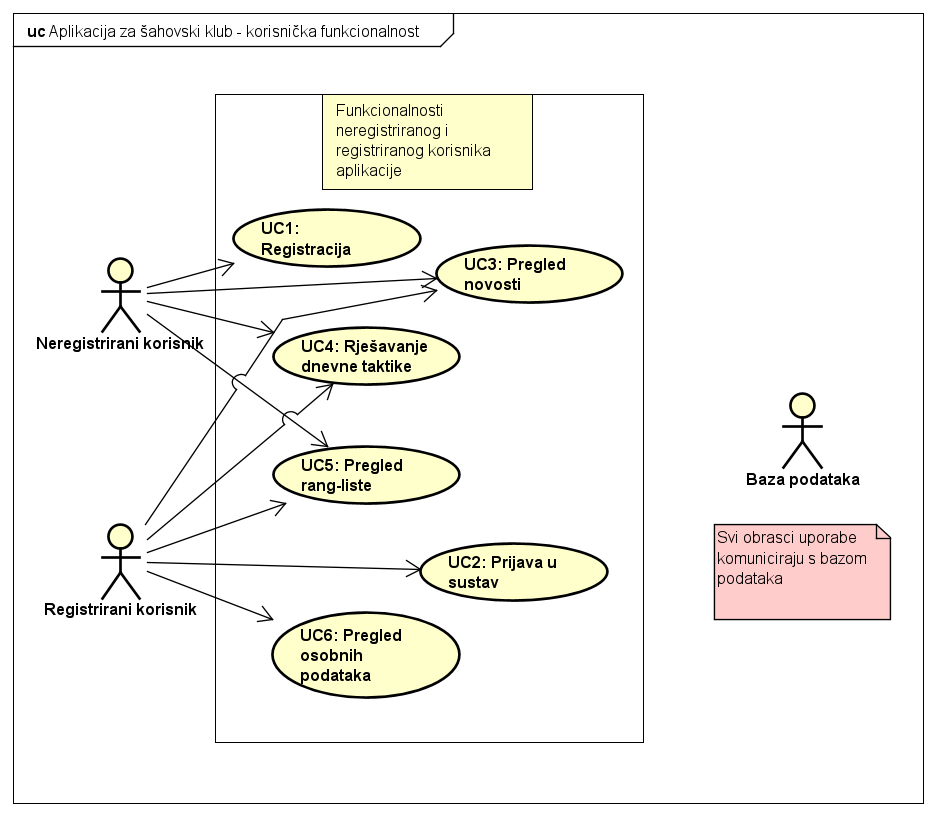
\includegraphics[width=\columnwidth]{korisnik_uc_dijagram}
		\begin{center}
			\textit{Slika 3.1: Dijagram obrasca uporabe, korisnička funkcionalnost}
		\end{center}
		\eject
		
		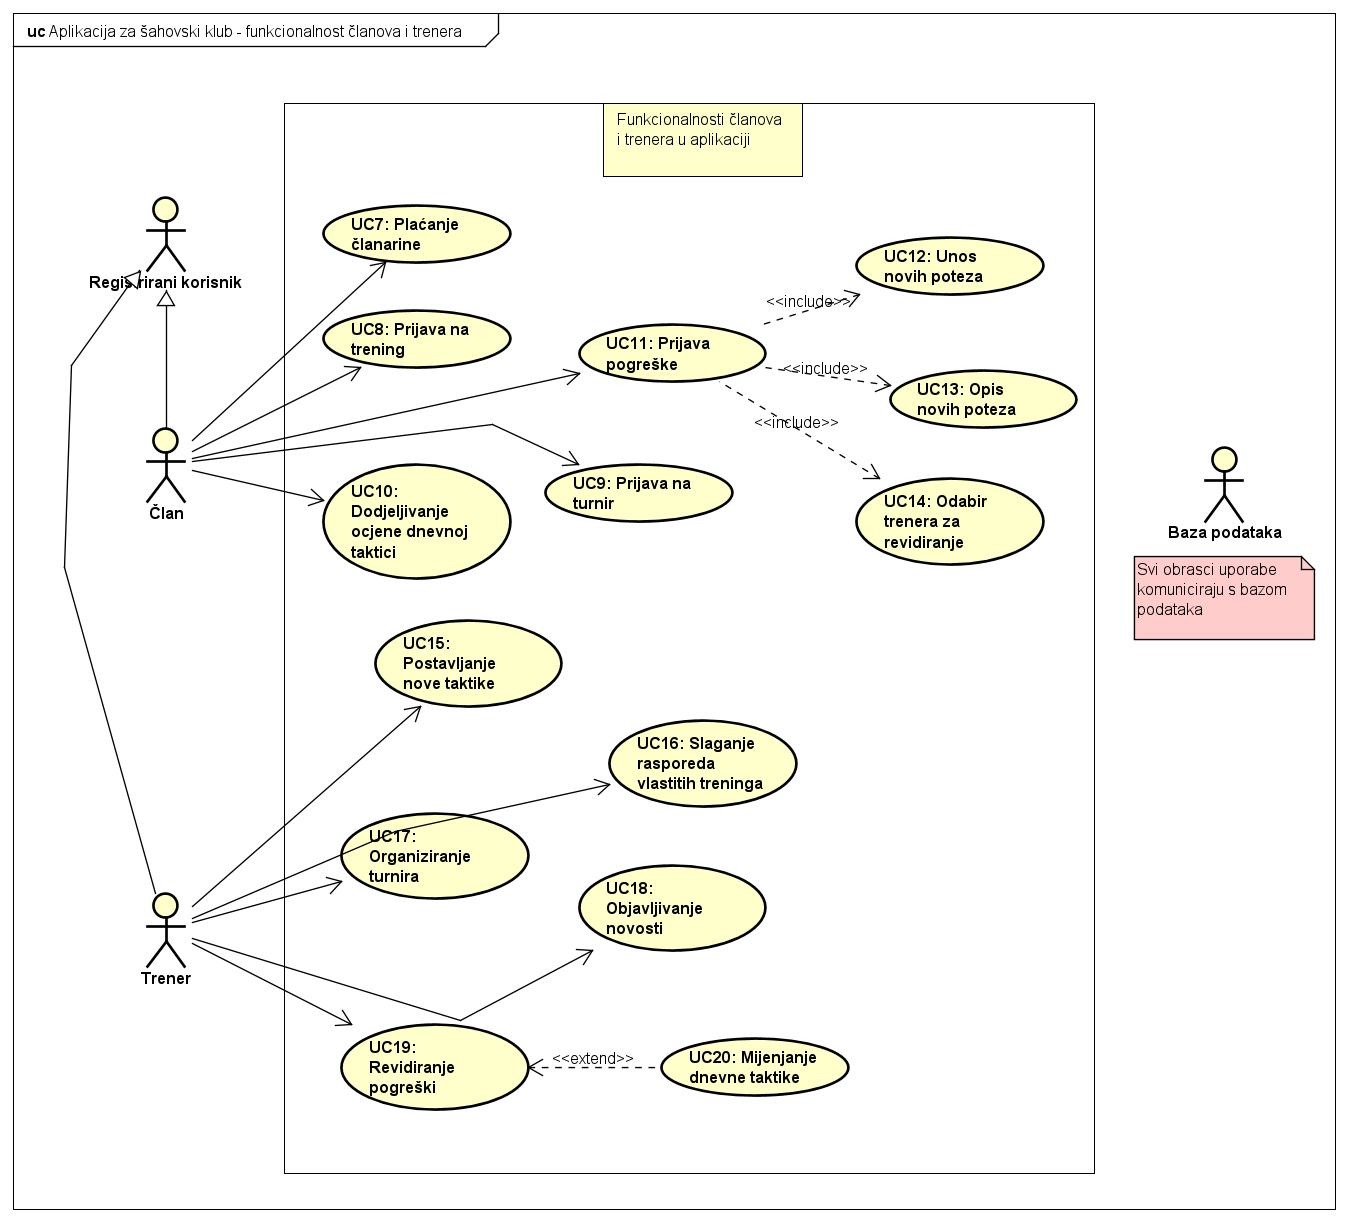
\includegraphics[width=\columnwidth]{clanovi_i_treneri_uc_dijagram}
		\begin{center}
			\textit{Slika 3.2: Dijagram obrasca uporabe, funkcionalnost člana i trenera}
		\end{center}
		\eject
		
		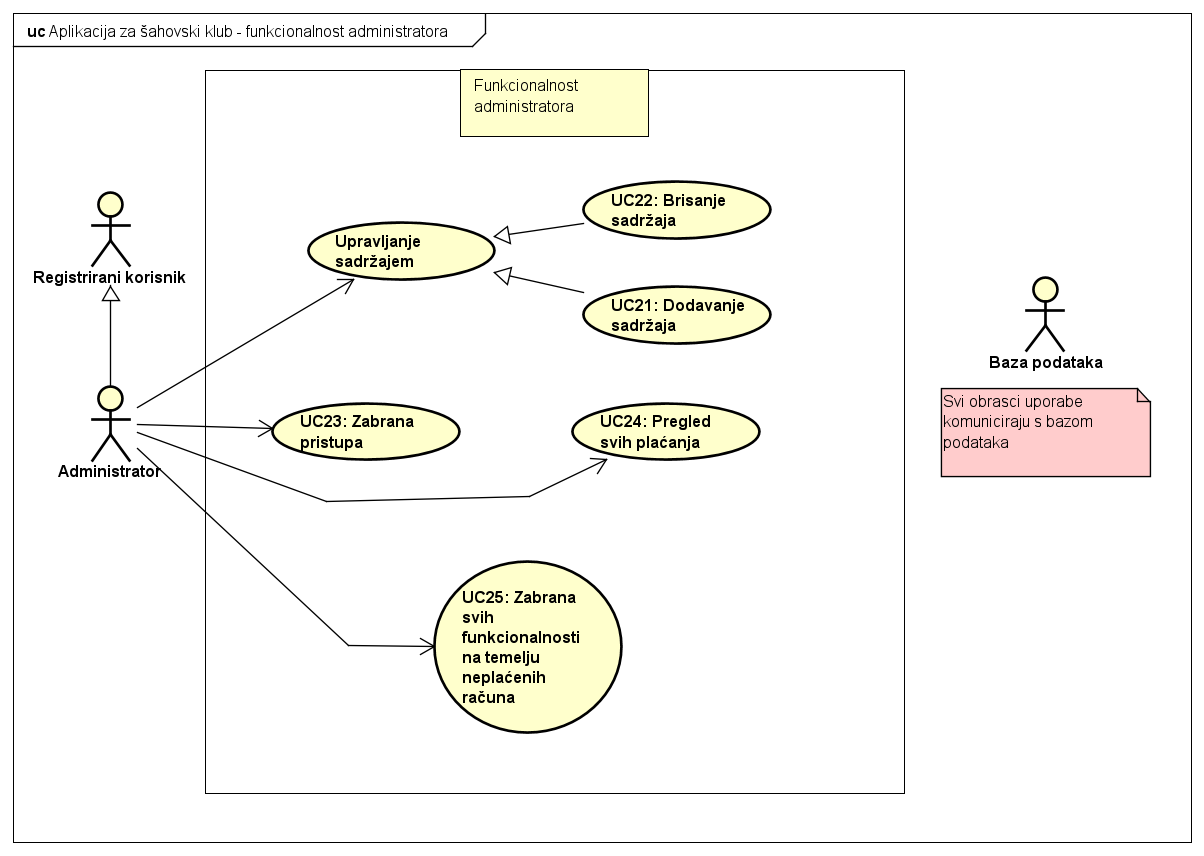
\includegraphics[width=\columnwidth]{administrator_uc_dijagram}
		\begin{center}
			\textit{Slika 3.3: Dijagram obrasca uporabe, funkcionalnost administratora}
		\end{center}
		\eject
		
		\subsubsection{Sekvencijski dijagrami}
		\textbf{Obrazac uporabe UC4 - Rješavanje dnevne taktike}\\
		Kad član pokrene rješavanje dnevne taktike, poslužitelj započinje mjeriti vrijeme, a nakon toga u bazu podataka prosljeduje izmjereno vrijeme odnosno ishod rješavanja dnevne taktike.
		Aplikacija uz to kreira težinsku rang listu članova na temelju povijensog učinka u rješavanju taktika, izmjerenog vremena za pojedini član te težine dnevne taktike.
		Ako član zamijeti pogrešku u dnevnoj taktici to prijavljuje unoseći nove poteze i opis novih poteza, zatim svaka prijavljena pogreška odlazi na revidiranje proizvoljno odabranom treneru. Ako se trener složi s novim rješenjem, ono se mora promijeniti na navedenoj taktici i automatski se moraju revidirati rang liste pri čemu se dodjeljuju bodovi onim članovima koji su ponudili točno rješenje, a uklanjaju onima koji su ponudili staro rješenje.
		\eject
		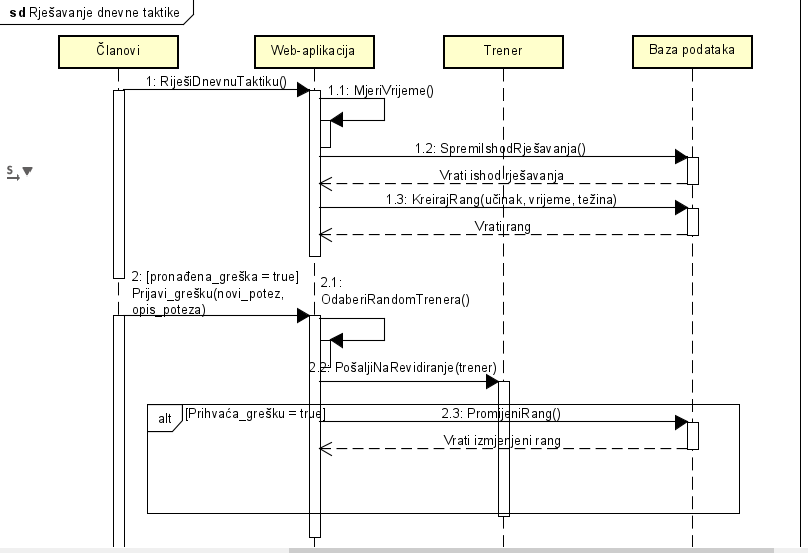
\includegraphics[width=\columnwidth]{rjesavanje_dnevnih_taktika}
		\begin{center}
			\textit{Slika 3.4: Sekvencijski dijagram za UC4}
		\end{center}
		\eject
		\textbf{Obrazac uporabe UC17 - Organiziranje turnira}\\
		Trener šalje zahtjev za pregled slobodnih termina kako bi mogao odabrati termin kada će se održati turnir. Poslužitelj dohvaća slobodne termine i prikazuje ih. Nakon što trener odabere termin, provjerava se ispravnost te se sprema odabir u bazu podataka nakon čega se prikazuje poruka koja ukazuje na uspješan odabir i rezervaciju termina. Trener može opcionalno promijeniti određene pojedinosti turnira. Ukoliko se na to odluči, trener šalje zahtjev za izmjenu pojedinosti. Poslužitelj dohvaća dosad određene pojedinosti treneru na izmjenu. Nakon što trener izmjeni željene pojedinosti, one se spremaju u bazu podataka. Na kraju se prikazuje poruka koja ukazuje na uspješnu izmjenu pojedinosti.
		\eject
		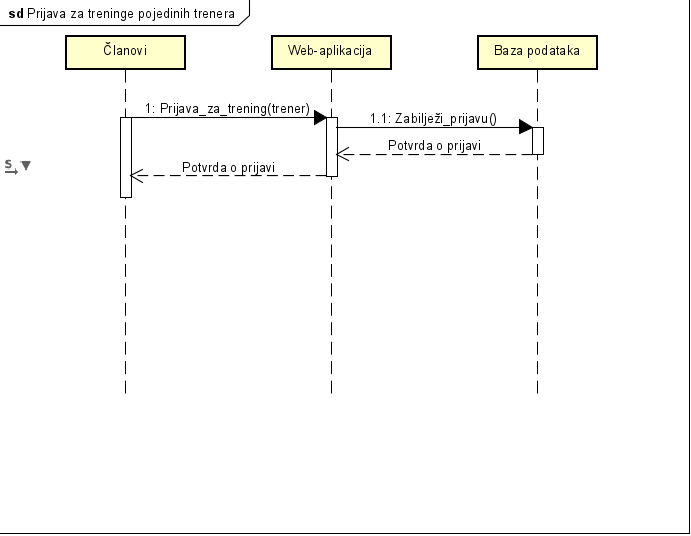
\includegraphics[width=\columnwidth]{prijava_za_treninge}
		\begin{center}
			\textit{Slika 3.5: Sekvencijski dijagram za UC17}
		\end{center}
		\eject
		\textbf{Obrazac uporabe UC24 - Pregled svih plaćanja}\\
		Administrator šalje zahtjev poslužitelju za prikaz transakcija pojedinog člana. Poslužitelj pristupa bazi podataka, dohvaća tražene transakcije i prikazuje ih. Ako transakcije ne postoje ili nisu provedene u cijelosti, administrator može članu zabraniti pristup svim funkcionalnostima aplikacije osim uplate članarine.
		\eject
		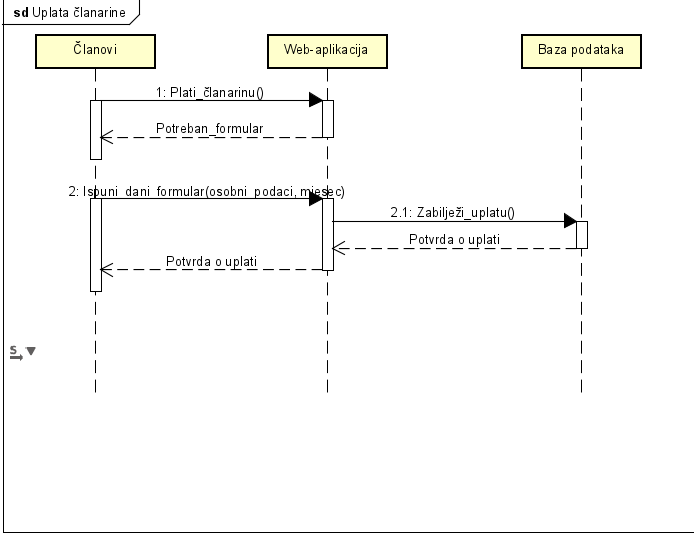
\includegraphics[width=\columnwidth]{uplata_clanarine}
		\begin{center}
			\textit{Slika 3.6: Sekvencijski dijagram za UC24}
		\end{center}
		\eject
		\subsection{Ostali zahtjevi}
		\begin{packed_enum}
			\item Sustav mora omogućiti paralelno korištenje aplikacije više korisnika u isto vrijeme bez ikakvih međusobnih interferencija
			\item Aplikacija mora biti maksimalno responzivna, korisnik ne smije puno čekati na odgovor ili prikaz sadržaja od strane sustava
			\item Sustav treba biti intuitivan i jednostavan za korištenje
			\item Neispravno korištenje ne smije rezultirati narušavanjem funkcionalnosti
			\item Korisnik treba biti spriječen pristupu određenih dijelova aplikacije ukoliko nije ovlašten
			\item Valute unutar sustava prikazane su u Eurima
			\item Nadogradnje sustava ne smiju narušavati postojeće funkcionalnosti sustava
			\item Pristup aplikaciji mora biti omogućen iz javne mreže
			\item Ukoliko je korisniku zabranjen pristup odlukom administratora, ne smije imati nikakve mogućnosti korištenja i treba biti obaviješten o tome, a ukoliko je zabranjen pristup zbog neplaćenih računa, treba mu biti sve ograničeno osim plaćanja računa
			\eject
		\end{packed_enum}
		
		\section{Arhitektura i dizajn sustava}
		\subsection{Opis arhitekture sustava}
		Arhitektura sustava može se podijeliti na 3 dijela:
		\begin{packed_enum}
			\item Prikaz web aplikacije korisniku (front-end)
			\item Web poslužitelj (back-end)
			\item Baza podataka
		\end{packed_enum}
	
		Našem proizvodu pristupa se putem web preglednika. Putem web preglednika, naša web aplikacija napisana u svojim programskim jezicima se prevodi u oblik koji je korisniku jasniji i prirodniji. To korisniku omogućuje korištenje svih funkcionalnosti naše aplikacije.\\
		Web poslužitelj temelj je rada naše aplikacije. On prima zahtjeve poslane od strane korisnika te vraća informacije koje je korisnik zatražio. Također, poslužitelj ima pristup bazi podataka u kojoj su pohranjeni svi podaci relevantni za rad naše aplikacije. Više o bazi podataka možete pročitati u poglavlju 4.2 (Baza podataka). Komunikacija između korisnika i poslužitelja odvija se pomoću HTTP protokola.\\
		Web aplikacija je korisniku prikazana na način da mu se omogući što lakši rad i interakcija s mogućnostima same aplikacije. Odabirom jedne od ponuđenih opcija na stranici, web preglednik šalje zahtjeve za potrebnim podatcima i/ili resursima s web poslužitelja/baze podataka na što mu poslužitelj odgovara. Ukoliko nije došlo do nikakvih nepredviđenih poteškoća, korisniku se prikazuje zatraženi sadržaj.
		Front-end naše aplikacije razvijen je u JavaScriptu ili točnije Reactu, open-source JavaScript biblioteci koja se koristi za jednostavnije kreiranje korisničkih sučelja. Kao dodatnu pomoć u nekim dijelovima korišten je i CSS.
		Back-end naše aplikacije razvijen je u JavaScriptu.
		Baza podataka razvijena je u pgAdmin 4, GUI-u razvijen za upravljanje i korištenje PostgreSQL sustavom upravljanja bazi podataka. 
		Razvojno okruženje korišteno za razvoj back-end i front-end dijela aplikacije je Visual Studio Code.
		Arhitektura sustava modelirana je prema MVC konceptu. Taj koncept se sastoji od 3 dijela; modela koji kontrolira radom i pravilima aplikacije, prima podatke od controllera te upravlja podacima, viewa koji predstavlja bilo kakav grafički ili drugi prikaz podataka te controllera, komponente koja prima zahtjeve korisnika i prosljeđuje ih drugim dijelovima sustava.
		Osim do sada navedenih značajki, naš sustav koristi JWT tehnologiju prenošenja podataka u obliku JSON objekata. JWT je skraćeno od JSON Web Token, a u našoj aplikaciji se koriste 2 vrste tokena, access token i refresh token. Access token služi za pristup resursima, a vremenski je ograničen. Refresh token ima dulje vrijeme trajanja od access tokena te služi za pridruživanje novog access tokena korisniku nakon isteka prijašnjeg access tokena. Na taj način korisnik se ne mora ponovno prijavljivati u sustav, no nakon eventualnog refresh tokena, korisnik će ipak morati obaviti ponovnu prijavu u sustav. 
		
		\eject
		\subsection{Baza podataka}
		Za potrebe našeg sustava koristit ćemo relacijsku bazu podataka koja svojom strukturom olakšava modeliranje stvarnog svijeta. Gradivna jedinka baze je relacija, odnosno tablica koja je definirana svojim imenom i skupom atributa. Zadaća baze podataka je brza i jednostavna pohrana, izmjena i dohvat podataka za daljnju obradu.Baza podataka ove aplikacije sastoji se od sljedecih entiteta:
		
			\begin{packed_item}
			
			\item {Users}
			\item  {Training} 
			\item  {Tournament}
			\item  {Scheduled training}
			\item  {Scheduled tournament}
			\item  {News}
			\item  {Daily tactics}
			\item  {Score}
			\item  {Reported mistake}
			\item  {Membership}
		\end{packed_item} 
		
	\large \textbf{Opis tablica}\\
	
	\textbf{Users} Ovaj entitet sadržava sve važne informacije o korisniku aplikacije. Sadrži atribute: userID, role, name, surname, username, email i pwdHash. Ovaj entitet u vezi je \textit{One-to-Many} s entitetom Training, Tournament, scheduledTraining, scheduledTournament, News, dailyTactics, Membership, reportedMistake i Score preko jedinstvenog identifikatora korisnika.
		
		
		
\setlength{\arrayrulewidth}{0.5mm}
\setlength{\tabcolsep}{10pt}
\renewcommand{\arraystretch}{1.5}		
		


	
	\begin{center}
    \begin{tabular}{ | l | l | l | p{5cm} |}
    \hline
    \multicolumn{3}{|c|}{Users}  \\ \hline
   \cellcolor{green!25}userID & INT & jedinstveni identifikator korisnika\\ \hline
    role & VARCHAR & uloga korisnika (trainer, member, admin)\\ \hline
    same & VARCHAR & ime korisnika \\ \hline
    surname & VARCHAR & prezime korisnika\\\hline
   email & VARCHAR & e-mail adresa korisnika\\ \hline
   pwdHash & INT & hash lozinke\\ \hline
    \end{tabular}
\end{center}
\eject

\textbf{Training} Ovaj entitet sadržava sve važne informacije o šahovskom treningu pojedinog trenera. Sadrži atribute: trainingID, trainerID, trainingStartTimeDate i trainingDurationMin. Ovaj entitet u vezi je \textit{Many-to-One} sa entitetom Users preko jedinstvenog identifikatora korisnika i \textit{One-to-Many} sa entitetom scheduledTraining.
		\\






  \begin{center}
    \begin{tabular}{ | l | l | l | p{5cm} |}
    \hline
    \multicolumn{3}{|c|}{Training}  \\ \hline
   \cellcolor{green!25}trainingID & INT & jedinstveni identifikator treninga \\ \hline  
   \cellcolor{blue!15}trainerID & INT & jedinstveni identifikator trenera \\ \hline
      trainingStartTimeDate  & TIMESTAMP & vrijeme početka treninga \\ \hline
    trainingDurationMin & INT & trajanje treninga \\ \hline
    \end{tabular}
\end{center}    
\bigskip
\bigskip
\bigskip


\textbf{Tournament} Ovaj entitet sadržava sve važne informacije o šahovskom turniru. Sadrži atribute: tournamentID, trainerID, tournamentStartTimeDate, tournamentDurationMin i participantsNo. Ovaj entitet u vezi je \textit{Many-to-One} sa entitetom Users preko jedinstvenog identifikatora korisnika i \textit{One-to-Many} sa entitetom scheduledTournament.
		\\
		
		
		

	\begin{center}
      \begin{tabular}{ | l | l | l | p{5cm} |}
    \hline
    \multicolumn{3}{|c|}{Tournament}  \\ \hline
    \cellcolor{green!25}tournamentID  & INT & jedinstveni identifikator turnira\\ \hline
    \cellcolor{blue!15}trainerID & INT & identifikator trenera \\ \hline
      tournamentStartTimeDate  &  TIMESTAMP  & vrijeme početka turnira \\ \hline
    tournamentDurationMin & INT & trajanje turnira\\\hline
    participantsNo   & INT & broj natjecatelja\\ \hline
    \end{tabular}
\end{center}
	\eject
	
	
	
	
	
	\textbf{scheduledTournament} Pomoću ovog entiteta zapisujemo koji član je prijavljen na koji turnir. Sadrži atribute: memberID i tournamentID. Ovaj entitet u vezi je \textit{Many-to-One} sa entitetom Tournament preko jedinstvenog identifikatora turnira i \textit{Many-to-One} sa entitetom Users preko jedinstvenog identifikatora korisnika.
		\\
		\bigskip
	
	
\begin{center}
    \begin{tabular}{ | l | l | l | p{5cm} |}
    \hline
    \multicolumn{3}{|c|}{scheduledTournament}  \\ \hline
   \cellcolor{green!25}memberID & INT & jedinstveni identifikator člana \\ \hline
    \cellcolor{green!25}tournamentID & INT & jedinstveni identifikator turnira \\ \hline
    \end{tabular}
\end{center}
\bigskip
\bigskip


\textbf{scheduledTraining} Pomoću ovog entiteta zapisujemo koji član je prijavljen na koje treninge. Sadrži atribute: memberID i trainingID. Ovaj entitet u vezi je \textit{Many-to-One} sa entitetom Training preko jedinstvenog identifikatora treninga i \textit{Many-to-One} sa entitetom Users preko jedinstvenog identifikatora korisnika.
		\\



\begin{center}
    \begin{tabular}{ | l | l | l | p{5cm} |}
    \hline
    \multicolumn{3}{|c|}{scheduledTraining}  \\ \hline
   \cellcolor{green!25}memberID & INT & jedinstveni identifikator člana \\ \hline
    \cellcolor{green!25}tournamentID & INT & jedinstveni identifikator trninga \\ \hline 
    \end{tabular}
\end{center}
\bigskip
\bigskip


\textbf{News} Ovaj entitet sadržava sve važne informacije o objavljenoj novosti. Sadrži atribute: newsID, trainerID i content. Ovaj entitet u vezi je \textit{Many-to-One} sa entitetom Users preko jedinstvenog identifikatora korisnika.
		\\



\begin{center}
    \begin{tabular}{ | l | l | l | p{5cm} |}
    \hline
    \multicolumn{3}{|c|}{News}  \\ \hline
   \cellcolor{green!25}newsID & INT & jedinstveni identifikator novosti \\ \hline
    \cellcolor{blue!15}trainerID & INT & jedinstveni identifikator trenera \\ \hline
    content & VARCHAR & sadržaj novosti \\ \hline 
    \end{tabular}
\end{center}





\textbf{dailyTactics} Ovaj entitet sadržava sve važne informacije o dnevnoj taktici. Sadrži atribute: tacticID, trainerID, content i solution. Ovaj entitet u vezi je \textit{Many-to-One} sa entitetom Users preko jedinstvenog identifikatora korisnika, \textit{One-to-Many} sa entitetima reportedMistake i Score.
		\\



\begin{center}
    \begin{tabular}{ | l | l | l | p{5cm} |}
    \hline
    \multicolumn{3}{|c|}{dailyTactics}  \\ \hline
   \cellcolor{green!25}tacticID & INT & jedinstveni identifikator dnevne taktike \\ \hline
    \cellcolor{blue!15}trainerID & INT & jedinstveni identifikator trenera \\ \hline
   content & VARCHAR & opis dnevnog zadatka \\ \hline 
    solution & VARCHAR & opis rješenja \\ \hline 
    \end{tabular}
\end{center}
\bigskip
\bigskip



\textbf{Score} Pomoću ovog entiteta zapisujemo uspjeh rješavanja dnevne taktike. Sadrži atribute: memberID, tacticID, solvingTime i accuracy. Ovaj entitet u vezi je \textit{Many-to-One} sa entitetom Users preko jedinstvenog identifikatora korisnika i \textit{Many-to-One} sa entitetom dailyTactics preko jedinstvenog identifikatora dnevne taktike.
		\\



\begin{center}
    \begin{tabular}{ | l | l | l | p{5cm} |}
    \hline
    \multicolumn{3}{|c|}{Score}  \\ \hline
   \cellcolor{green!25}memberID & INT & jedinstveni identifikator člana \\ \hline
    \cellcolor{blue!15}tacticID & INT & jedinstveni identifikator dnevne taktike \\ \hline
    solvingTime & TIME & vrijeme rješavanja\\ \hline 
    accuracy & FLOAT & točnost rješenja\\ \hline
    \end{tabular}
\end{center}
\eject



\textbf{reportedMistake} Pomoću ovog entiteta zapisujemo prijavljenu pogrešku dnevne taktike. Sadrži atribute: memberID, tacticID, trainerID, preposedMove, moveDescription i isFixed. Ovaj entitet u vezi je \textit{Many-to-One} sa entitetom Users preko jedinstvenog identifikatora korisnika i \textit{Many-to-One} sa entitetom dailyTactics preko jedinstvenog identifikatora dnevne taktike.
		\\
		



\begin{center}
    \begin{tabular}{ | l | l | l | p{5cm} |}
    \hline
    \multicolumn{3}{|c|}{reportedMistake}  \\ \hline
   \cellcolor{green!25}memberID & INT & jedinstveni identifikator člana \\ \hline
    \cellcolor{green!25}tacticID & INT & jedinstveni identifikator dnevne taktike \\ \hline
     \cellcolor{blue!15}trainerID & INT & jedinstveni identifikator trenera \\ \hline
    preposedMove & VARCHAR & predloženo rješenje \\ \hline 
     moveDescription & VARCHAR & opis predloženog rješenja \\ \hline
     isFixed & BOOLEAN & oznaka je li greška rješena\\ \hline
    \end{tabular}
\end{center}
\bigskip
\bigskip



\textbf{Membership} Pomoću ovog entiteta zapisujemo plaćanje članarine članova. Sadrži atribute: memberID, periodStart, periodEnd i isPaid. Ovaj entitet u vezi je \textit{Many-to-One} sa entitetom Users preko jedinstvenog identifikatora korisnika.
		\\



\begin{center}
    \begin{tabular}{ | l | l | l | p{5cm} |}
    \hline
    \multicolumn{3}{|c|}{Membership}  \\ \hline
   \cellcolor{green!25}memberID & INT & jedinstveni identifikator člana \\ \hline
    periodStart & INT & početak peroda za koji se plaća članarina \\ \hline
    periodEnd & INT & kraj peroda za koji se plaća članarina \\ \hline
      isPaid & BOOLEAN & oznaka je li članarina plaćena\\ \hline
      
    \end{tabular}
\end{center}



	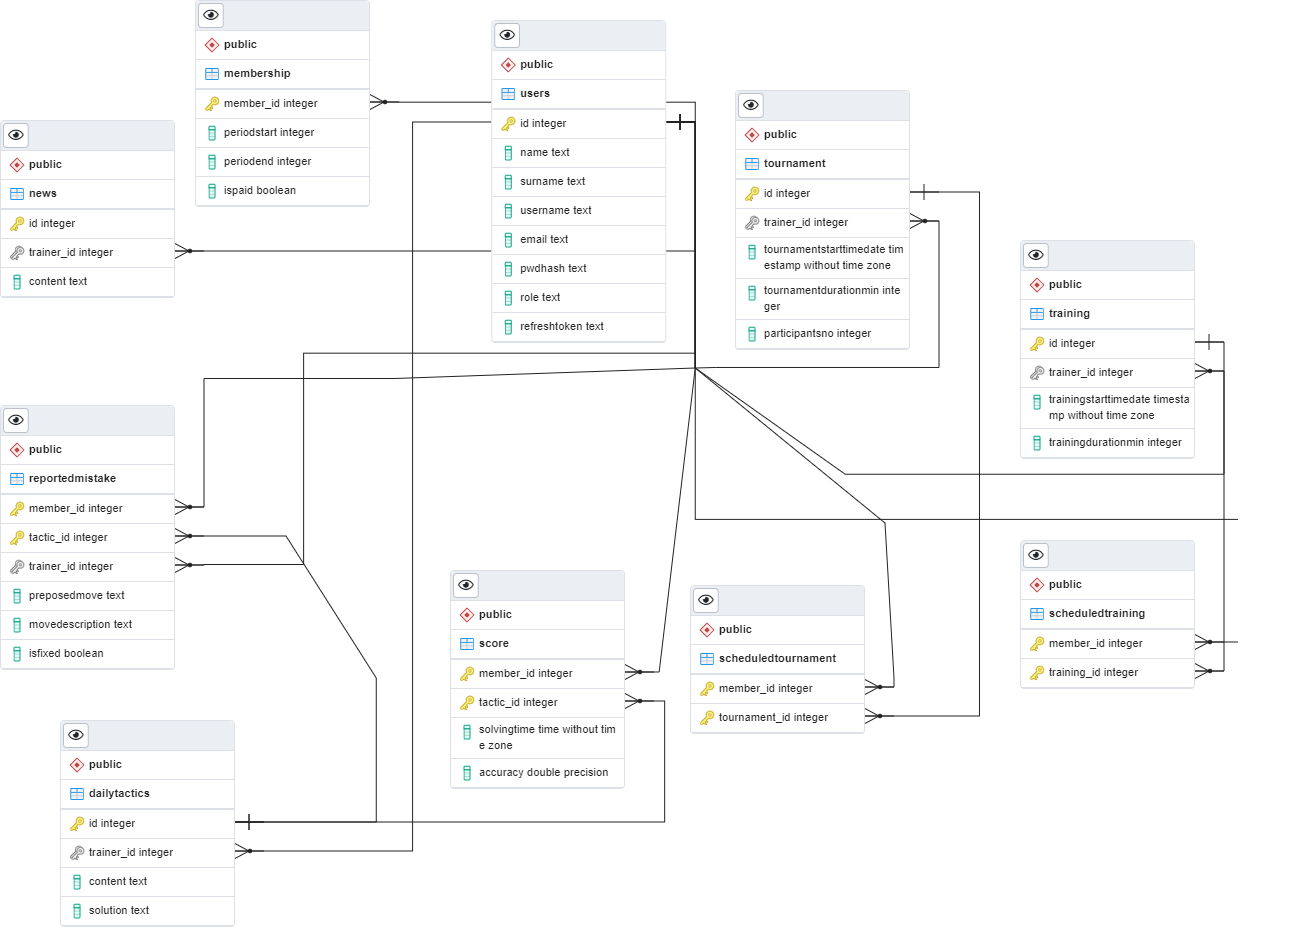
\includegraphics[width=\columnwidth]{ERbaze.png}
		\begin{center}
			\textit{E-R model baze podataka}
		\end{center}

\eject

	\subsection{Dijagram razreda}

	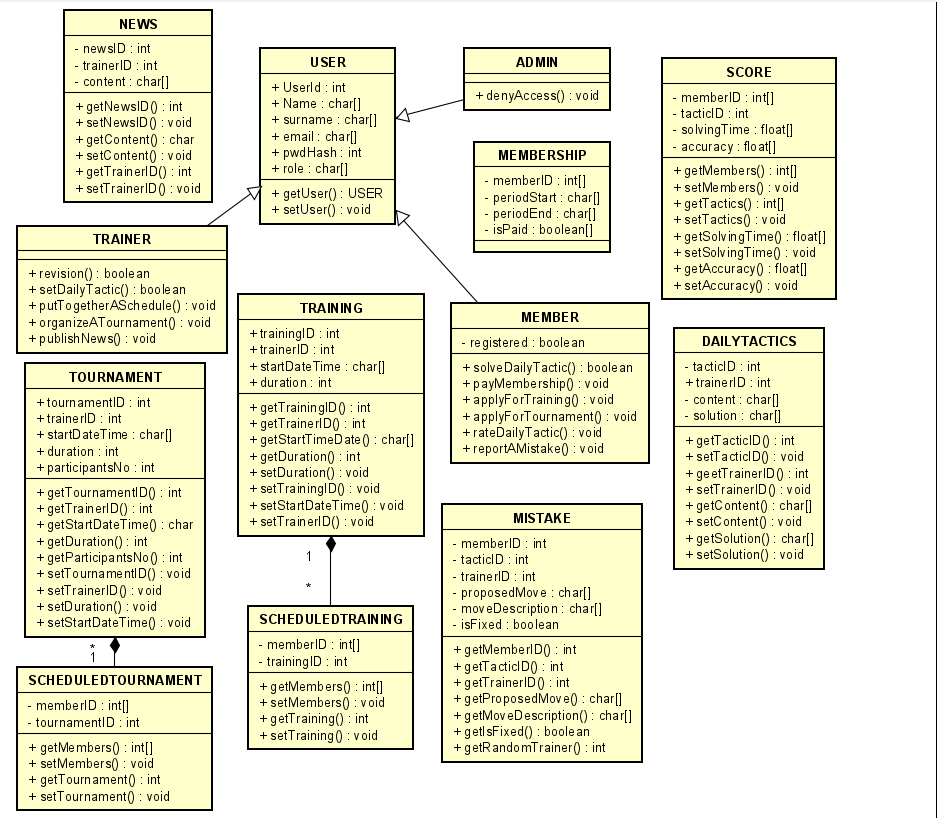
\includegraphics[width=\columnwidth]{slike/dijagramRazreda.PNG}
		\begin{center}
			\textit{Dijagram razreda}
		\end{center}


\end{document}